\begin{frame}[parent={ie:agenda}, hasnext=true, hasprev=false]
	\frametitle{Modelo de Benington}

	\begin{block:concept}{Definição}
		Modelo de produção em cascata, um dos primeiros (senão o primeiro) modelo de
		ciclo de vida para desenvolvimento de software~\cite{Benington:1983}.
	\end{block:concept}

	
	\begin{block:fact}{Contexto}
		\begin{itemize}
			\item Projeto para desenvolvimento do sistema de controle de defesa do
			espaço aéreo norte-americano (SAGE).
			
			\item Desenvolvido pelo MIT Lincoln Laboratory (centro de pesquisa do DoD
			norte-americano e, na época, terceirizado da IBM para desenvolver o SAGE).
			
			\item 1950.
		\end{itemize}
	\end{block:fact}
	
	\note{
 		\begin{itemize}
			\item SAGE = \textbf{S}emi-\textbf{A}utomatic \textbf{G}round \textbf{E}nvironment
			\\Praticamente um sistema Guerra nas Estrelas.
				
	 		\item Mais informações em:
	 		\begin{itemize}
	 			\item http://en.wikipedia.org/wiki/Semi-Automatic\_Ground\_Environment
	 			\item http://en.wikipedia.org/wiki/AN/FSQ-7\_Combat\_Direction\_Central
	 			\item http://en.wikipedia.org/wiki/MIT\_Lincoln\_Laboratory
	 		\end{itemize}
 		\end{itemize}
	}
\end{frame}


\begin{frame}[hasnext=true, hasprev=true]
	\frametitle{Modelo de Benington}

	\begin{columns}
		\column{.45\textwidth}
		\begin{block:fact}{}
			\centering
			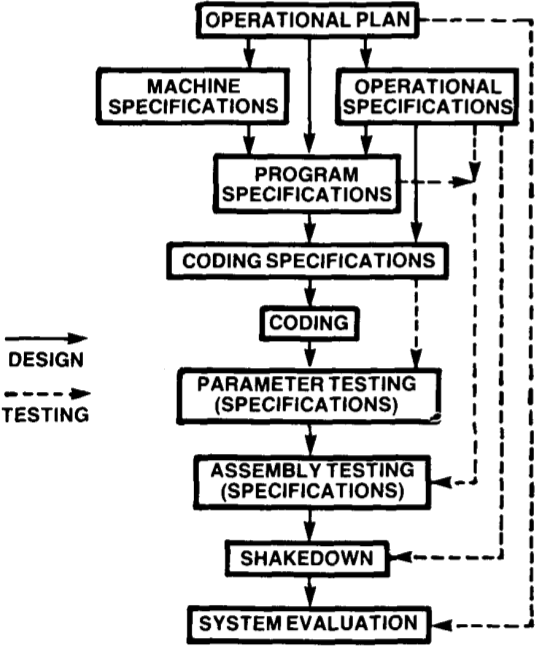
\includegraphics[width=\textwidth]{software-engineering/project-management/process/sdlc/benington/Benington software life-cycle model.png}
		\end{block:fact}	

		\column{.5\textwidth}
		\begin{block:fact}{}
			\small
			\begin{itemize}
			 \item Plano operacional
			 \item Especificação operacional
			 \item Especificação dos programas
			 \item Especificação da codificação do programa
			 \item Codificação
			 \item Teste funcional do programa
			 \item Teste funcional do sistema
			 \item Teste de aceitação do sistema
			\end{itemize}
		\end{block:fact}
	\end{columns}

	\note{
		\begin{itemize}
			\item Fases:
			\begin{itemize}
				\item Plano operacional: requisitos do projeto.
				\item Especificação operacional: requisitos da interface entre hardware
				e software.
				\item Especificação dos programas (comunicação entre programas e
				escalonamento/compartilhamento de tempo entre programas).
				\item Especificação da codificação do programa: definição da entrada e
				saída de cada programa.
			\end{itemize}
		
			\item Lembre-se: programas muito estruturados, com comunicação limitada
			entre funções e pouca dependência de dados. Isto permitia/facilitava o
			desenvolvimento em cascata.
		\end{itemize}
	}
\end{frame}


\begin{frame}[hasnext=false, hasprev=true]
	\frametitle{Modelo de Benington}

	\begin{block:fact}{Fatores de sucesso}
		 \begin{itemize}
				\item Funcionários eram todos engenheiros e trabalham como tal (racionalização,
				documentação, gerenciamento).
				
				\item Desenvolvimento iterativo (grande granularidade, mas ainda iterativo).
		\end{itemize}
	\end{block:fact}
		
	\begin{block:fact}{Lições aprendidas}
		\begin{itemize}
			\item Se pudessem, teriam dado passos menores (iterações menos complexas).
			
			\item Por mais que sejam observadas as experiências de outros, no final das
			contas criar um software grande é como criar uma família.
			
			\item Entretanto, melhorou substancialmente o desenvolvimento
			(em especial para design e teste).
		\end{itemize}
	\end{block:fact}

	\note{
		\begin{itemize}
			\item Na primeira iteração, eles construiram uma versão de 35.000 instruções
			para uma arquitetura computacional. Na segunda iteração, eles construiram
			uma versão de 100.000 instruções para \textbf{outra} arquitetura. Em suma,
			foram dois grandes passos de uma só vez (e isso teve um custo elevado).
			
			\item Analogia com criar uma família: no final das contas, você precisa fazer as coisas
			por si, aprender as opções únicas que você tem, trabalhar com os problemas
			inesperados e, com sorte, terminar tão bem quanto aqueles que fazem essas
			coisas (cuidar da família) há muito tempo.
		\end{itemize}
	}
\end{frame}